\documentclass[lettersize,onecolumn,journal]{IEEEtran}
\usepackage{amsmath,amsfonts}
\usepackage{algorithmic}
\usepackage{titling}
\usepackage{algorithm}
\usepackage{array}
\usepackage[caption=false,font=normalsize,labelfont=sf,textfont=sf]{subfig}
\usepackage{textcomp}
\usepackage{listings}
\lstset{basicstyle=\ttfamily, keywordstyle=\bfseries}
\usepackage{stfloats}
\usepackage{url}
\usepackage{verbatim}
\usepackage{graphicx}
\usepackage[nospace,compress,sort]{cite}
\hyphenation{op-tical net-works semi-conduc-tor IEEE-Xplore}
\usepackage{graphicx}
\usepackage{color}
\usepackage{amsmath,amssymb}
\usepackage{booktabs}
\usepackage{multirow}
\usepackage{wrapfig}
\usepackage{url}
\usepackage{ragged2e}
\usepackage{amsfonts,dcolumn}
\usepackage{makecell}
\usepackage{array}

\usepackage{caption}
\captionsetup[table]{labelfont={sc,small},textfont={sc,small},justification=centering,labelsep=newline}
\captionsetup[figure]{labelfont={sc,small},textfont={sc,small},justification=centering,labelsep=newline}

\lstset{language=Python, literate={symbol_1}{symbol_l}1 {symbol_2}{simbol_2}1 }


\begin{document}
	
	%----------------------------
	\title{[CSE299(1) - Group\#6] Project Proposal: Home Healthcare \& Diagnostic Center Management System}
	\date{28th July 2026 / Summer 2026}
	\author{Md Mehrab Hossain Khandoker 2311511042\\
		Nafsin Nasama Salmee 2311776642\\
		Mohammed Mushfiq Syed 2232295042\\
		Yousuf Jamil 2321210642\\
		Email Addresses: \{mehrab.khandoker, nafsin.salmee, mohammed.syed, yousuf.jamil.232\}@nothsouth.edu}
	\maketitle
	
	\section{Introduction}
	
	\subsection{Project Overview}
	Access to timely, efficient, and comprehensive healthcare services remains a critical challenge globally, particularly in developing and densely populated regions \cite{telemedicine_homecare}. Traditional healthcare delivery relies heavily on physical hospital visits, which often result in prolonged waiting times, increased financial burden, heightened risk of nosocomial infections, and severe logistical challenges for vulnerable demographics—including elderly, chronically ill, pediatric, and post-surgical patients \cite{telemedicine_homecare}.
	
	To address these systemic inefficiencies, the \textbf{Home Healthcare \& Diagnostic Center Management System (HHDMS)} introduces a centralized, multi-role digital ecosystem designed to bridge the gap between primary clinical care, specialized medical services, field nursing, home caregiving, and mobile diagnostic operations \cite{srs2026}. By combining call center dispatching, real-time field logistics, electronic medical record (EMR) management, dynamic scheduling, mobile point-of-care diagnostics, and telehealth capabilities into a unified architecture, HHDMS transforms home healthcare from a fragmented service model into an integrated, end-to-end clinical workflow \cite{srs2026}.
	
	\subsection{Problem Statement}
	Despite the growing demand for decentralized and home-based medical services, existing healthcare systems suffer from severe operational limitations \cite{telemedicine_homecare}:
	\begin{itemize}
		\item \textbf{Fragmented Operational Silos:} Patient intakes, doctor teleconsultations, home nursing visits, and diagnostic testing currently operate as disconnected services \cite{srs2026}. This lack of integration leads to lost medical records, repeated clinical evaluations, and poor care continuity across the patient lifecycle \cite{srs2026}.
		\item \textbf{Inadequate Dispatch and Field Visibility:} Traditional home healthcare management relies on manual scheduling without real-time tracking \cite{zandbergen2009accuracy}. Operators and patients lack visibility into provider locations, dynamic Estimated Time of Arrival (ETA) predictions, or verifiable geofenced visit attendance \cite{zandbergen2009accuracy, osrm_routing}.
		\item \textbf{Inaccessible Mobile Point-of-Care Diagnostics:} Conducting advanced diagnostic imaging—such as bedside Ultrasonography (USG) or Digital X-Rays—outside fixed hospital settings remains technically isolated \cite{pacs2001}. Without native Digital Imaging and Communications in Medicine (DICOM) support, specialists are unable to remotely review, measure, and annotate diagnostic scans in real time \cite{dicom2021, cornerstone3d}.
		\item \textbf{Heterogeneous Workflows and Security Gaps:} Managing diverse clinical professionals (e.g., MBBS triage doctors, 11 categories of specialists, adult and pediatric nurses) alongside non-clinical personnel (e.g., long-term caregivers, nutritionists, diagnostic technicians) under a unified, role-aware security and permission framework presents a complex operational challenge \cite{rbac_standard}.
	\end{itemize}
	
	\subsection{Objectives}
	The primary objective of HHDMS is to design, develop, and deploy a robust, scalable, and multi-tenant digital healthcare management system \cite{srs2026}. Specific goals include:
	\begin{enumerate}
		\item \textbf{Centralized Lifecycle Management:} Establish a streamlined intake pipeline via call center ticket dispatch, structured referral chains, and unified Medical Record Numbers (MRN) to preserve complete chronological patient history \cite{srs2026}.
		\item \textbf{Real-Time Field Optimization:} Implement automated resource allocation, device GPS tracking (30-second polling), route estimation, and dynamic 100-meter geofenced check-in/out verification for field clinicians, nurses, and caregivers \cite{zandbergen2009accuracy, haversine_formula, osrm_routing}.
		\item \textbf{Advanced Point-of-Care Diagnostic Capabilities:} Enable bedside DICOM imaging capture for mobile ultrasound and X-ray services, backed by an interactive web-based image viewer for remote specialist analysis and reporting \cite{dicom2021, pacs2001, cornerstone3d}.
		\item \textbf{Integrated Telehealth and Communication:} Provide secure, low-latency video/audio teleconsultations, instant messaging, and automated real-time notification alerts across mobile and web platforms \cite{fette2011websocket, agorawebrtc}.
	\end{enumerate}
	
	\subsection{Scope of the System}
	HHDMS encompasses a cross-platform solution comprising a high-performance backend REST API and WebSocket engine, an administrative web application, and a feature-rich mobile client \cite{srs2026, nestjs_framework, nextjs_app_router}. The platform supports more than ten distinct operational roles, including Call Center Agents, General Practitioners (MBBS), Specialist Doctors, Nurses, Caregivers, Nutritionists, Diagnostic Technicians, System Administrators, and Patients \cite{srs2026, rbac_standard}. Through this comprehensive framework, HHDMS governs every phase of home healthcare—from primary contact and dynamic triage to treatment planning, point-of-care diagnostic delivery, and automated billing \cite{srs2026, accv2016}.
	
	\section{Background and Related Work}
	
	\subsection{Background and Domain Context}
	Over recent years, the global healthcare ecosystem has undergone a paradigm shift from traditional, centralized hospital visits to decentralized, patient-centric care delivery models \cite{telemedicine_homecare}. Home healthcare and telehealth solutions have emerged as critical infrastructures to alleviate hospital congestion, reduce healthcare delivery costs, and provide accessible, continuous care to patients—particularly elderly individuals, chronically ill patients, and post-surgical cases \cite{telemedicine_homecare}. In regions such as Bangladesh, where urban traffic, limited mobility, and overburdened healthcare facilities present significant barriers to timely clinical interventions, home-delivered clinical and non-clinical healthcare services offer a practical solution \cite{srs2026}.
	
	A modern home healthcare infrastructure requires more than basic teleconsultations; it demands a unified platform capable of orchestrating complex multi-disciplinary clinical operations \cite{srs2026}. This includes coordinating general practitioner (MBBS) first-response triage, multi-specialty consultations (spanning 11 clinical specialties), adult and pediatric nursing care, specialized caregiver support (male, female, child care across flexible shift durations), and mobile diagnostic testing such as portable Ultrasonography (USG) and Digital X-Ray \cite{srs2026}. Managing this spectrum of services necessitates an integrated digital platform that harmonizes centralized call center dispatch, real-time field asset tracking, electronic medical record (EMR) management, diagnostic imaging, dynamic scheduling, and automated billing \cite{srs2026}.
	
	\subsection{Challenges in Existing Home Healthcare Systems}
	Despite the growing demand for home-based medical care, traditional home healthcare management is hindered by operational fragmentation, communication bottlenecks, and technology gaps \cite{telemedicine_homecare}:
	
	\begin{itemize}
		\item \textbf{Fragmented Patient Journey \& Lack of Care Continuity:} Existing solutions often separate primary triage, specialist referrals, nursing care, and diagnostic results into isolated silos \cite{srs2026}. Without a unified Medical Record Number (MRN) and structured referral chain, health records become lost across transfers, preventing doctors, specialists, and field care providers from obtaining a complete chronological patient context \cite{srs2026}.
		\item \textbf{Inadequate Real-Time Dispatch and Visibility:} Dispatched healthcare staff (nurses, caregivers, doctors, and diagnostic technicians) frequently operate with minimal oversight \cite{zandbergen2009accuracy}. Conventional platforms lack real-time Global Positioning System (GPS) tracking, automated Estimated Time of Arrival (ETA) calculation, and geofenced visit verification, leaving both call center operators and patients without visibility regarding provider dispatch and arrival times \cite{zandbergen2009accuracy, osrm_routing}.
		\item \textbf{Limited Diagnostic Integration at Home:} While standard telehealth apps provide audio or video consultations, they lack integration with point-of-care diagnostics \cite{pacs2001}. Conducting specialized ultrasound or X-ray examinations at a patient’s bedside requires native support for Digital Imaging and Communications in Medicine (DICOM) standards, enabling specialists to review, annotate, and interpret medical images remotely within the application pipeline \cite{dicom2021, cornerstone3d}.
		\item \textbf{Disconnected Clinical and Non-Clinical Workflows:} Managing clinical professionals (MBBS doctors, specialists) alongside non-clinical support personnel (caregivers logging daily hygiene/mobility activities) within a single security and permission architecture remains an open operational challenge \cite{rbac_standard}. Existing platforms rarely provide specialized interfaces tailored to specific roles—such as pediatric growth tracking, caregiver activity/condition reporting, or nutritionist anthropometric calculation \cite{who_child_growth}.
	\end{itemize}
	
	\subsection{Related Work \& Comparative Analysis}
	Existing digital healthcare platforms generally fall into three distinct categories, each with specific architectural and operational limitations when applied to comprehensive home healthcare management:
	
	\begin{table}[htbp]
		\centering
		\small
		\begin{tabular}{|>{\RaggedRight\arraybackslash}m{2.8cm}|>{\RaggedRight\arraybackslash}m{3.5cm}|>{\RaggedRight\arraybackslash}m{3.5cm}|>{\RaggedRight\arraybackslash}m{4.2cm}|}
			\hline
			\textbf{System Category} & \textbf{Core Functionality} & \textbf{System Strengths} & \textbf{Operational Gaps in Home Care} \\ \hline
			\textbf{Standard Telemedicine Apps} & Video/Audio teleconsultations, electronic prescriptions, basic appointment scheduling. & Fast onboarding, lightweight client requirements, direct doctor-patient interaction. & Lacks field staff dispatch, GPS tracking, home nursing/caregiver management, and portable diagnostic imaging workflows \cite{telemedicine_homecare}. \\ \hline
			\textbf{Hospital Information Systems (HIS/EMR)} & In-hospital bed management, inpatient/outpatient billing, laboratory information management systems (LIMS). & Robust clinical record storage, formal diagnostic catalog management, internal pharmacy tracking. & Designed strictly for fixed-location healthcare facilities; lacks field geofencing, real-time map tracking, offline mobile capability, and call-center ticket dispatches \cite{pacs2001}. \\ \hline
			\textbf{Standalone Dispatch / Logistics Systems} & Vehicle and field worker tracking, basic appointment booking, proof of arrival/delivery. & Real-time map visibility, automated route optimization, driver ETA updates. & Void of clinical capabilities: lacks ICD-10 diagnosis coding, drug interaction checking, DICOM imaging viewers, and multi-specialty clinical workflows \cite{who2016icd10, dicom2021}. \\ \hline
		\end{tabular}
		\vspace{0.5em}
		\caption{\scshape Comparative Analysis of Digital Healthcare System Categories}
		\label{tab:related_work}
	\end{table}
	
	The \textbf{Home Healthcare \& Diagnostic Center Management System (HHDMS)} bridges these gaps by combining clinical governance, diagnostic capability, and field logistics into a single centralized digital platform \cite{srs2026, accv2016}.
	
	\subsection{The Proposed Solution: HHDMS Overview}
	To resolve these domain limitations, \textbf{HHDMS} presents a centralized multi-role platform that governs the complete lifecycle of home healthcare delivery—from initial call center intake to field dispatch, clinical assessment, bedside diagnostics, remote specialist consultation, and finalized billing \cite{srs2026}.
	
	The system is architected as a distributed ecosystem comprising a \textbf{NestJS 11 REST \& Socket.IO backend API} \cite{nestjs_framework, fette2011websocket}, a \textbf{Next.js 16 App Router web dashboard} \cite{nextjs_app_router} (for call center agents, doctors, specialists, nutritionists, sonologists, and admins), and a \textbf{Jetpack Compose Android application} (for patients, field doctors, caregivers, and nurses):
	
	\begin{itemize}
		\item \textbf{Unified Multi-Role Triage \& Workflow:} Supports 10+ distinct user roles (Call Center Agents, MBBS Doctors, 11 Specialist categories, Adult/Pediatric Nurses, Nutritionists, Caregivers, Sonologists, X-Ray Technicians, System Admins, and Patients) operating under a single Role-Based Access Control (RBAC) mechanism \cite{srs2026, rbac_standard}.
		\item \textbf{Centralized Intake \& Care Chain Tracking:} Incoming calls auto-trigger caller lookup, patient registration with unique Medical Record Numbers (MRNs), and alphanumeric Ticket ID tracking across a unified care chain timeline \cite{srs2026}.
		\item \textbf{Real-Time Logistics \& Geofenced Dispatch:} Integrates device GPS tracking (30-second interval polling), OpenStreetMap \slash  OSRM routing, dynamic traffic-based ETA calculations, and automated 100-meter geofence check-in/out verification for field personnel \cite{zandbergen2009accuracy, haversine_formula, osrm_routing}.
		\item \textbf{Point-of-Care Diagnostic Capabilities:} Features portable ultrasound and X-ray study capture, DICOM image storage, and an interactive Cornerstone3D DICOM viewer allowing specialists to perform distance/ellipse measurements, annotations, and side-by-side image comparison directly within the browser \cite{dicom2021, pacs2001, cornerstone3d}.
		\item \textbf{Integrated Real-Time Communications:} Incorporates Socket.IO WebSockets for live chat and call signaling \cite{fette2011websocket}, Agora RTC SDK for low-latency WebRTC teleconsultations \cite{agorawebrtc}, Firebase Cloud Messaging (FCM) for urgent alerts, and automated Stripe/mobile banking payment integrations \cite{stripe2024api}.
	\end{itemize}
	
	\section{Problem Identification}
	
	\subsection{Domain-Specific Operational Bottlenecks}
	The delivery of home healthcare services involves a complex, highly dynamic interaction among call center operators, general practitioners, specialists, field staff, and patients \cite{srs2026}. Managing these operations manually or through unintegrated software applications introduces several severe operational bottlenecks \cite{srs2026}:
	
	\begin{itemize}
		\item \textbf{Call Center and Dispatch Inefficiencies:} Call center agents frequently lack real-time visibility into the availability, schedule, geographical location, and active workload of field healthcare personnel (doctors, nurses, caregivers, and technicians) \cite{srs2026}. This leads to delayed service assignment, manual phone call chains, prolonged patient wait times, and high rates of ticket dropped calls or misrouted requests \cite{srs2026}.
		\item \textbf{Lack of Real-Time Field Asset Tracking and Attendance Verification:} Once field staff are dispatched, healthcare administrators and patients have no reliable mechanism to track their location, monitor travel progress, or verify actual arrival times \cite{zandbergen2009accuracy}. Traditional attendance mechanisms rely on self-reported check-ins, which are prone to inaccuracies, time fraud, and an inability to provide dynamic Estimated Time of Arrival (ETA) updates \cite{zandbergen2009accuracy}.
		\item \textbf{Complex Duty Shift and Multi-Tier Pricing Management:} Home care support—ranging from short-term nursing procedures to 8-hour, 12-hour, or 24-hour caregiver shifts—requires intricate scheduling rules and differential pricing models based on duration, shift timing, gender preference, and service tier \cite{srs2026}. Standard administrative systems lack the flexibility to automate these dynamic billing and assignment structures without manual calculation errors \cite{srs2026}.
	\end{itemize}
	
	\subsection{Clinical Governance and Data Continuity Gaps}
	Healthcare delivery outside fixed medical facilities introduces substantial risks to clinical quality, patient safety, and medical record integrity \cite{telemedicine_homecare}:
	
	\begin{itemize}
		\item \textbf{Information Silos and Broken Referral Chains:} Patients receiving home care often transition through multiple providers—from an initial MBBS call center triage to field nursing, specialty consultations (e.g., Cardiology, Neurology, Pediatrics), and follow-up caregivers \cite{srs2026}. In existing systems, medical notes, physical assessment logs, and prescription histories are stored in disconnected formats, preventing specialists from accessing a continuous, chronological Medical Record Number (MRN) history \cite{srs2026}.
		\item \textbf{Role-Incompatible Assessment Interfaces:} Clinical data collection needs vary drastically across disciplines \cite{srs2026}. For example, pediatric nursing requires specialized WHO growth standard charting \cite{who_child_growth}, nutritionists require targeted body composition and intake metrics, and long-term caregivers require continuous activity-of-daily-living (ADL) logs \cite{srs2026}. Universal form templates fail to capture these distinct clinical requirements effectively \cite{srs2026}.
		\item \textbf{Unstructured Medication Management and Diagnostic Ordering:} Prescriptions and lab orders generated during home visits are frequently recorded as handwritten physical notes or unstructured text messages \cite{srs2026}. This creates high risks of drug interaction errors, transcription mistakes, missed diagnostic follow-ups, and an inability to maintain an auditable electronic audit trail \cite{who2016icd10}.
	\end{itemize}
	
	\subsection{Technical and Diagnostic Integration Constraints}
	Delivering bedside diagnostics and real-time remote consultations at home faces critical technical barriers \cite{srs2026}:
	
	\begin{itemize}
		\item \textbf{Isolation of Point-of-Care Diagnostic Imaging:} While portable Ultrasonography (USG) and Digital X-Ray devices permit home diagnostic testing, the captured medical imagery is rarely integrated into the patient’s central EMR in real time \cite{pacs2001}. Radiologists and sonologists must often physically receive files via non-compliant media or separate isolated systems, delaying urgent diagnostic reporting \cite{pacs2001}.
		\item \textbf{Absence of Web-Native DICOM Processing Tools:} Standard web and mobile applications lack embedded support for native Digital Imaging and Communications in Medicine (DICOM) rendering \cite{dicom2021}. Consequently, remote specialists are unable to perform essential clinical image manipulations—such as adjusting Window Width/Window Level (WW/WL), capturing length and angle measurements, or performing multi-frame video sequence playback—directly within their web browsers \cite{cornerstone3d}.
		\item \textbf{Communication Latency and Insecure Interoperability:} Real-time video teleconsultations, instant messaging, and system push notifications often run on disjointed third-party software \cite{fette2011websocket, agorawebrtc}. This creates latency issues during urgent triage, lacks synchronization with the central patient record, and introduces vulnerabilities regarding compliance with patient data privacy standards \cite{agorawebrtc}.
	\end{itemize}
	
	\subsection{Problem Summary}
	In summary, current home healthcare models are hindered by a fundamental disconnection between administrative dispatch, field logistics, multi-specialty clinical workflows, and bedside diagnostic imaging \cite{srs2026}. Without a unified platform that simultaneously resolves real-time dispatch tracking, role-specific clinical intake, web-native DICOM diagnostic analysis, and centralized EMR management, home healthcare delivery will remain inefficient, fragmented, and difficult to scale \cite{srs2026, accv2016}.
	
	\section{Solution Methodology}
	
	To address the operational, clinical, and technical challenges identified in home healthcare delivery, the \textbf{Home Healthcare \& Diagnostic Center Management System (HHDMS)} adopts a modular, domain-driven full-stack architecture \cite{srs2026}. The methodology combines cloud-native API design \cite{nestjs_framework}, real-time WebSocket communication \cite{fette2011websocket}, geofenced mobile asset tracking \cite{zandbergen2009accuracy, haversine_formula}, point-of-care DICOM diagnostic processing \cite{dicom2021, cornerstone3d}, and multi-tier Role-Based Access Control (RBAC) \cite{rbac_standard}.
	
	\subsection{System Architecture and Tech Stack}
	The HHDMS infrastructure is organized into a three-tier architecture comprising a centralized backend core, a reactive web management console, and a native mobile platform:
	
	\begin{figure}[htbp]
		\centering
		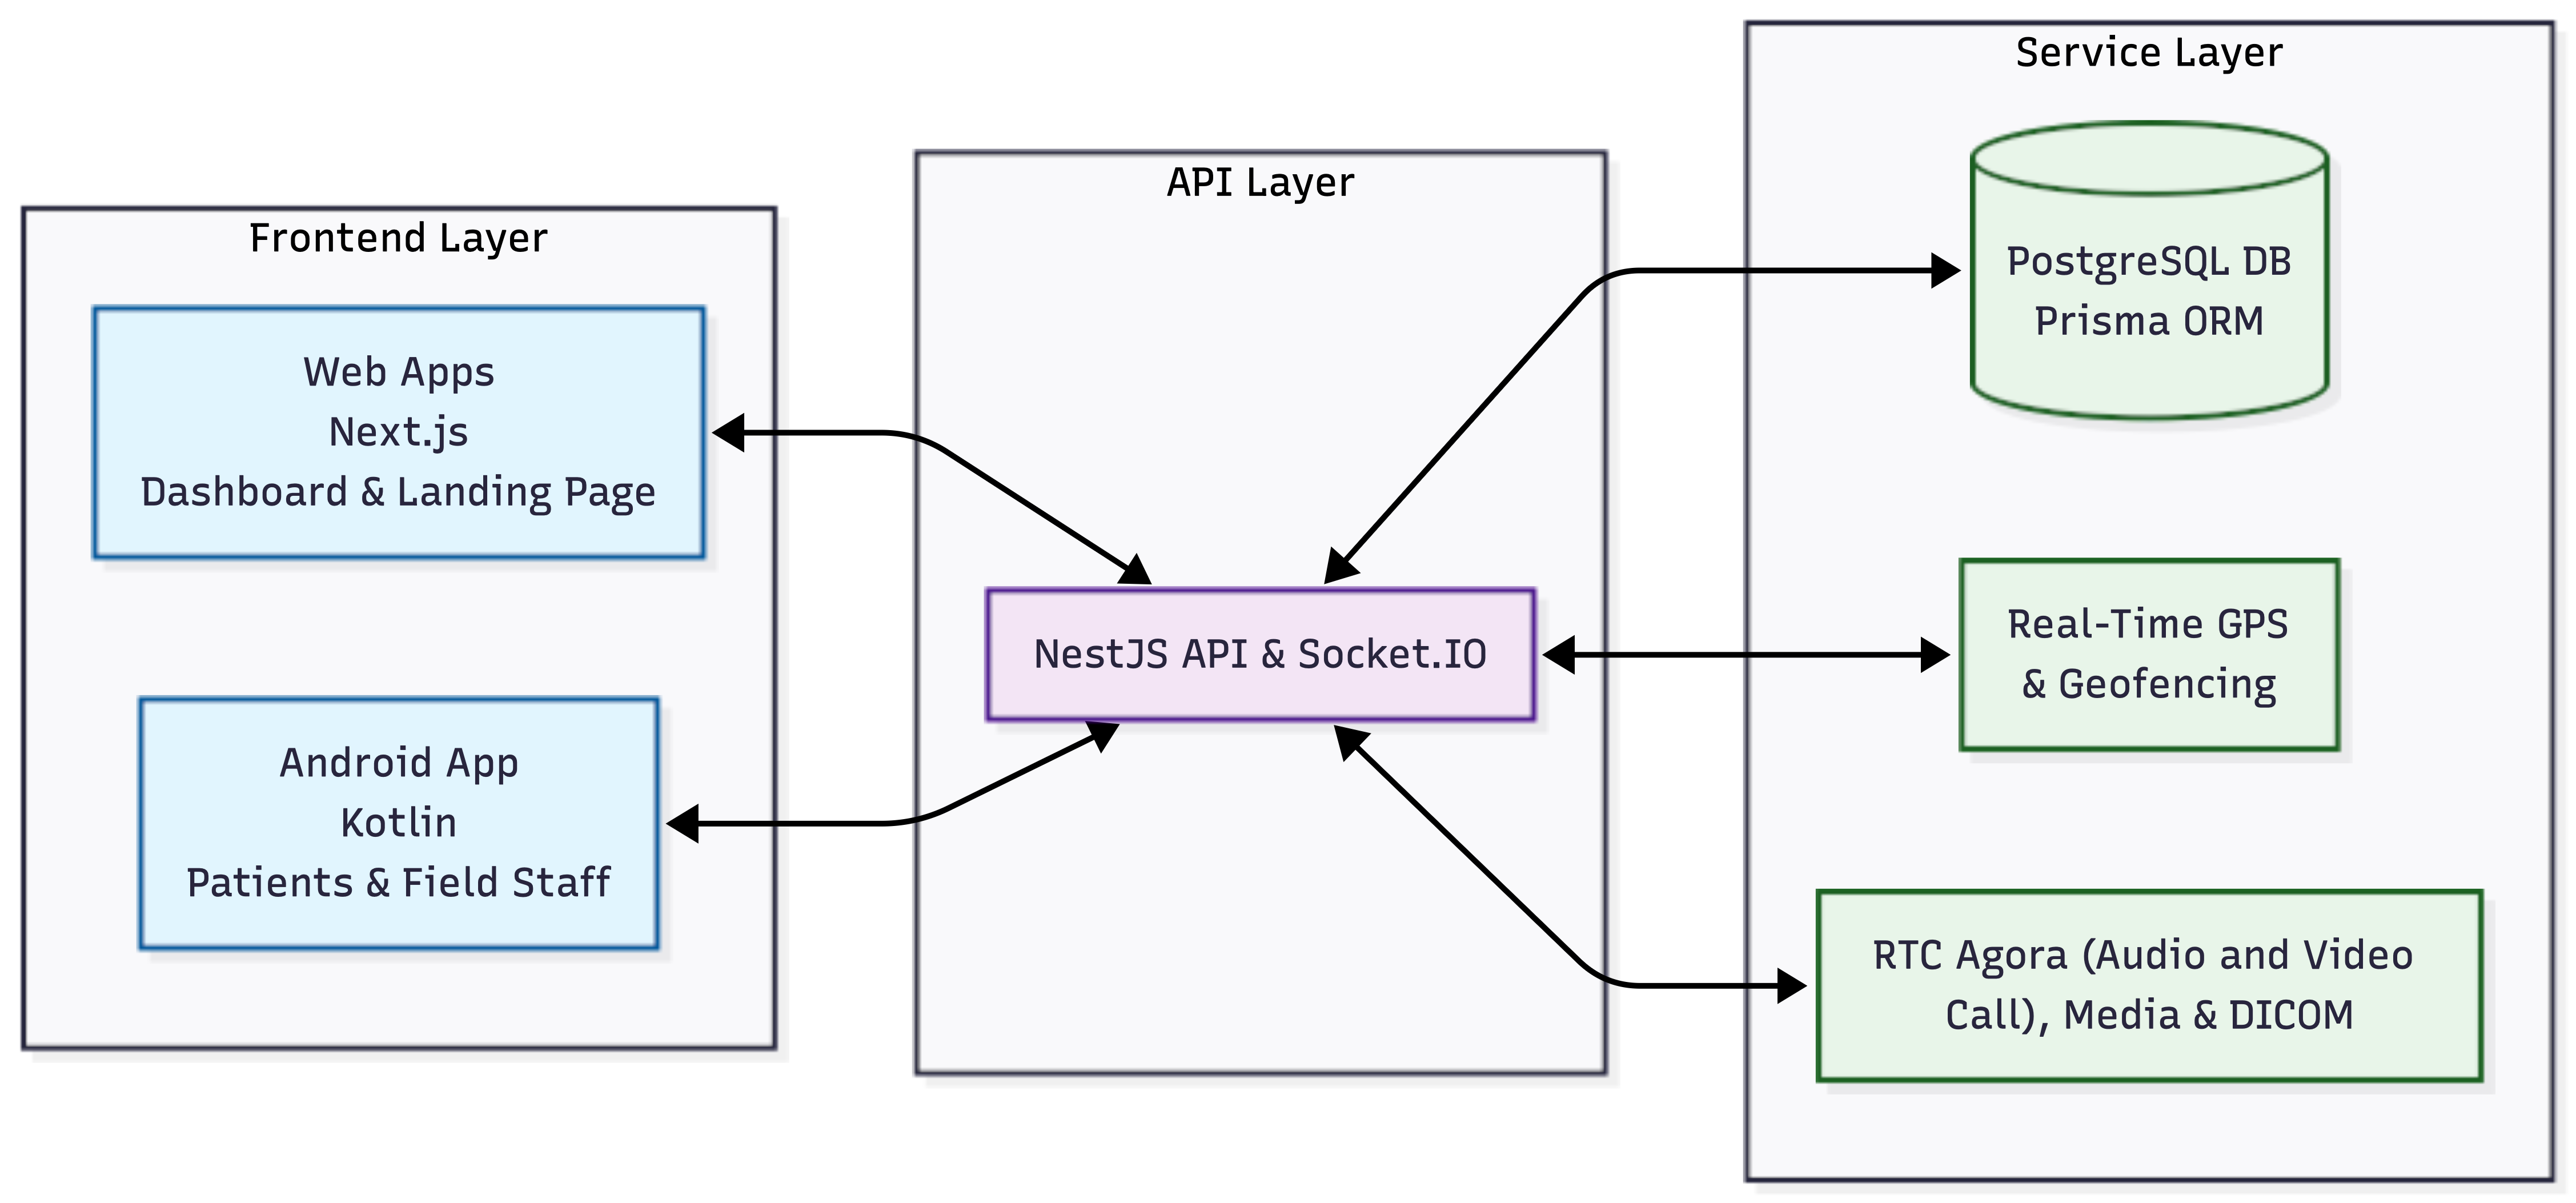
\includegraphics[width=0.9\linewidth]{project_flow.png}
		\vspace{0.5em}
		\caption{\scshape System Architecture of HHDMS showing communication flows between FRONTEND clients, NESTJS backend API, POSTGRESQL storage, and real-time integration modules.}
		\label{fig:hhdms_architecture}
	\end{figure}
	
	\begin{itemize}
		\item \textbf{Backend Core (NestJS 11 \& Socket.IO):} Built on Node.js using TypeScript, the backend provides structured modular controllers, services, and gateways \cite{nestjs_framework}. Inter-service communications run on RESTful endpoints for CRUD operations and bi-directional Socket.IO WebSockets for real-time events \cite{fette2011websocket}.
		\item \textbf{Database \& Persistence (PostgreSQL \& Prisma ORM):} Relational data persistence is managed using PostgreSQL, abstracted via Prisma ORM for type-safe schema definitions, automated migrations, and complex dynamic relational queries \cite{srs2026}.
		\item \textbf{Administrative Web Client (Next.js 16 App Router):} A modern React-based web dashboard designed for Call Center Agents, Doctors, Specialists, Sonologists, Nutritionists, and System Admins, utilizing Tailwind CSS for dynamic UI rendering \cite{nextjs_app_router}.
		\item \textbf{Mobile Field Client (Android - Jetpack Compose):} A native Android application built using Kotlin and Jetpack Compose, utilized by Patients, Field Doctors, Nurses, and Caregivers for real-time order processing, vitals submission, and GPS tracking \cite{srs2026}.
	\end{itemize}
	
	\subsection{Centralized Call Center Intake and Lifecycle Pipeline}
	The core operational workflow begins at the centralized Call Center, which orchestrates the complete patient care chain \cite{srs2026}:
	
	\begin{enumerate}
		\item \textbf{Caller Intake and Registration:} When a request arrives, call center agents perform real-time phone number lookups. New patients are registered with a permanent, unique Medical Record Number (MRN) \cite{srs2026}.
		\item \textbf{Ticket Dispatch Lifecycle:} Each service request triggers an alphanumeric Ticket ID tracked across distinct status states: \texttt{PENDING}, \texttt{ASSIGNED}, \texttt{EN\_ROUTE}, \texttt{IN\_PROGRESS}, \texttt{COMPLETED}, and \texttt{CANCELLED} \cite{srs2026}.
		\item \textbf{Structured Referral Chains:} Triage MBBS doctors evaluate patient requests via voice or video calls. If secondary specialist consultations, diagnostic imaging, or nursing procedures are required, the triage doctor generates structured internal referrals attached to the active ticket, maintaining complete historical context \cite{srs2026, who2016icd10}.
	\end{enumerate}
	
	\begin{figure*}[htbp]
		\centering
		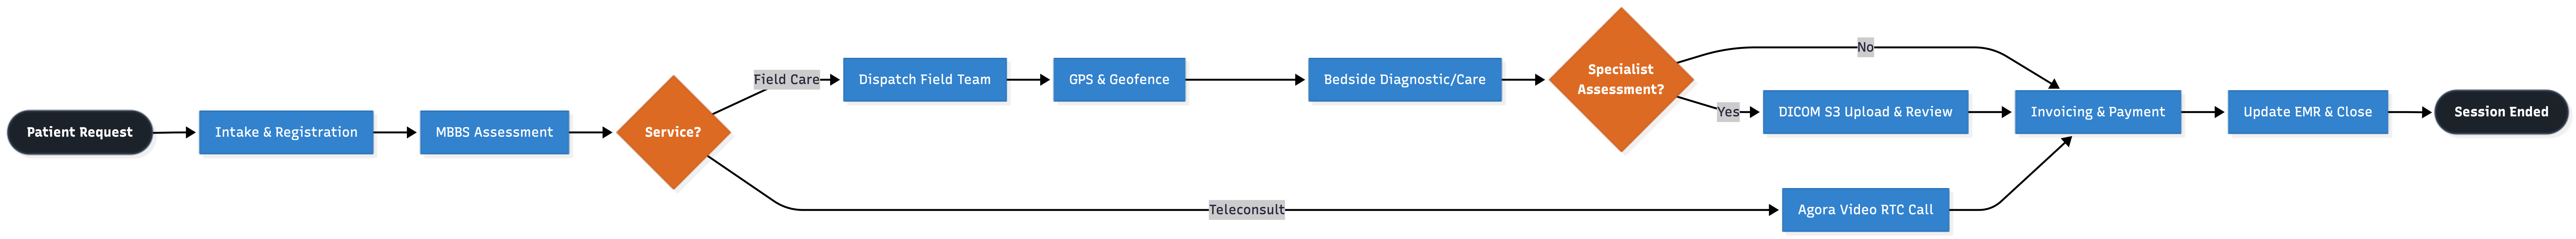
\includegraphics[width=0.98\linewidth]{patient_flow.png}
		\vspace{0.5em}
		\caption{\scshape End-to-End Patient Journey and Service Execution Flow within the HHDMS Platform.}
		\label{fig:patient_flow}
	\end{figure*}
	
	\subsection{Real-Time Field Logistics and Geofenced Dispatch}
	To guarantee operational transparency and prevent attendance fraud, HHDMS implements real-time location and spatial algorithms \cite{zandbergen2009accuracy, haversine_formula}:
	
	\begin{itemize}
		\item \textbf{Background GPS Polling:} Dispatched field personnel (doctors, nurses, caregivers, technicians) run a persistent background service on their mobile devices, emitting high-precision GPS coordinates every 30 seconds via WebSockets \cite{fette2011websocket, zandbergen2009accuracy}.
		\item \textbf{Routing and Traffic-Aware ETA:} Coordinate streams are processed using OpenStreetMap\slash OSRM APIs to generate accurate, traffic-adjusted Estimated Time of Arrival (ETA) values displayed simultaneously to call center operators and waiting patients \cite{osrm_routing}.
		\item \textbf{Automated Geofence Verification:} The system computes the Haversine distance $d$ between the worker's current coordinates $(\phi_1, \lambda_1)$ and the patient's registered home coordinates $(\phi_2, \lambda_2)$ \cite{haversine_formula}:
		\begin{equation}
			d = 2r \arcsin \left( \sqrt{\sin^2\left(\frac{\phi_2 - \phi_1}{2}\right) + \cos(\phi_1)\cos(\phi_2)\sin^2\left(\frac{\lambda_2 - \lambda_1}{2}\right)} \right)
		\end{equation}
		where $r$ represents Earth's radius ($6,371 \text{ km}$). A virtual geofence radius $R_{gf} = 100 \text{ meters}$ is enforced; the field staff mobile interface automatically unlocks the "Start Visit" button only when $d \le R_{gf}$ \cite{haversine_formula}.
	\end{itemize}
	
	\subsection{Bedside Point-of-Care DICOM Diagnostic Workflow}
	To solve the issue of diagnostic isolation during home visits, HHDMS integrates a specialized point-of-care imaging workflow \cite{dicom2021, pacs2001}:
	
	\begin{enumerate}
		\item \textbf{Field Imaging Capture:} Diagnostic technicians (Sonologists and X-Ray Technicians) conduct bedside scans using portable digital ultrasonography or digital X-ray equipment \cite{dicom2021}.
		\item \textbf{DICOM Ingestion:} Raw diagnostic files structured under the Digital Imaging and Communications in Medicine (DICOM) standard are uploaded directly to secure object storage via the mobile interface \cite{dicom2021, pacs2001}. Metadata (patient ID, study date, modality, series instance UID) is parsed and indexed into PostgreSQL \cite{dicom2021}.
		\item \textbf{Interactive Web DICOM Viewer:} Specialists access a browser-based viewer powered by Cornerstone3D \cite{cornerstone3d}. The viewer supports interactive image manipulations, including Window Width / Window Level (WW/WL) adjustments, dynamic zoom, linear distance measurements, elliptical area calculations, and multi-frame cine-loop playback for ultrasound videos \cite{cornerstone3d}.
		\item \textbf{Remote Radiographic Reporting:} Specialists complete and sign formal diagnostic reports directly within the application, automatically notifying the referring physician and updating the patient's master EMR file \cite{pacs2001}.
	\end{enumerate}
	
	\subsection{Role-Aware Clinical Workflows and Real-Time Telecommunication}
	The platform enforces granular Role-Based Access Control (RBAC) across 10+ operational roles, delivering custom interfaces tailored to each discipline \cite{rbac_standard}:
	
	\begin{itemize}
		\item \textbf{Specialized Clinical Interfaces:} Adult nurses access vitals logging screens; pediatric nurses utilize WHO growth chart plotting tools \cite{who_child_growth}; nutritionists utilize automated BMI and daily caloric allowance calculators; caregivers log daily Activities of Daily Living (ADL) checklists \cite{srs2026}.
		\item \textbf{Real-Time RTC and Messaging:} Real-time video and audio teleconsultations are powered by the Agora WebRTC SDK \cite{agorawebrtc}, ensuring sub-second latency across varying network bandwidths. Instant chat messaging is facilitated via WebSockets \cite{fette2011websocket}, supported by Firebase Cloud Messaging (FCM) push notifications for time-critical alerts.
		\item \textbf{Automated Financial Management:} The system dynamically calculates shift billing based on hourly tiers, procedure complexity, and provider grade, generating automated invoices integrated with online payment gateways (Stripe and local mobile banking) \cite{stripe2024api}.
	\end{itemize}
	
	\section{Expected Timeline}
	
	The development and deployment of the \textbf{Home Healthcare \& Diagnostic Center Management System (HHDMS)} is structured over an intensive 6-week execution cycle \cite{srs2026}. The timeline is strategically mapped around five sequential weekly progress milestones leading directly into the final project submission and demonstration \cite{srs2026}.
	
	\subsection*{\textbf{Detailed Weekly Milestone Breakdown:}}
	
	\begin{table}[htbp]
		\centering
		\small
		\begin{tabular}{|>{\RaggedRight\arraybackslash}m{2.5cm}|>{\RaggedRight\arraybackslash}m{5cm}|>{\RaggedRight\arraybackslash}m{6.5cm}|}
			\hline
			\textbf{Phase / Milestone} & \textbf{Core Engineering Focus} & \textbf{Target Deliverables \& Demo Scope} \\ \hline
			\textbf{Week 1: Demo 1} & Architecture Setup, Core Auth, \& Patient Intake & Environment configuration, PostgreSQL schema migration, NestJS JWT RBAC engine, and Call Center Agent dashboard for initial patient registration and ticket creation \cite{srs2026, nestjs_framework, rbac_standard}. \\ \hline
			\textbf{Week 2: Demo 2} & Dynamic Triage, Referrals, \& Nurse/Caregiver Modules & Triage MBBS consultation module, internal referral routing, shift-based assignment engine, and specialized interfaces for Adult/Pediatric Nursing and Caregivers \cite{srs2026, who2016icd10, who_child_growth}. \\ \hline
			\textbf{Week 3: Demo 3} & Real-Time Logistics \& Geofenced Tracking & Native Android background location service (30s polling), Socket.IO live map integration, OSRM dynamic ETA computation, and automated 100m geofence visit verification \cite{zandbergen2009accuracy, fette2011websocket, haversine_formula, osrm_routing}. \\ \hline
			\textbf{Week 4: Demo 4} & Mobile Diagnostic Capture \& Interactive DICOM Viewer & Bedside ultrasound/X-ray DICOM upload, S3-compatible cloud storage ingestion, metadata parsing, and web-native Cornerstone3D viewer with WW/WL and measurement tools \cite{dicom2021, pacs2001, cornerstone3d}. \\ \hline
			\textbf{Week 5: Demo 5} & Real-Time RTC, Telehealth, \& Billing Systems & Agora WebRTC video/audio integration, Socket.IO instant messaging, Firebase push notifications, and automated dynamic invoicing with Stripe/mobile banking gateways \cite{fette2011websocket, stripe2024api, agorawebrtc}. \\ \hline
			\textbf{Week 6: Final Demo} & End-to-End Testing, Security Audit, \& Deployment & System integration testing, end-to-end scenario validation, role performance optimization, production containerization (Docker/Nginx), and Final Project Presentation \cite{srs2026}. \\ \hline
		\end{tabular}
		\vspace{0.5em}
		\caption{Project Execution Roadmap and Weekly Demo Deliverables}
		\label{tab:project_timeline}
	\end{table}
	
	\subsubsection{Week 1: Core Platform Setup \& Triage Pipeline (Weekly Demo 1)}
	\begin{itemize}
		\item Environment initialization: Setup NestJS 11 backend, Next.js 16 web application, and Android Jetpack Compose codebase repositories \cite{nestjs_framework, nextjs_app_router}.
		\item Database Modeling: Design PostgreSQL relational schema via Prisma ORM covering Users, Roles, Tickets, Patients, and EMR records \cite{srs2026}.
		\item Authentication \& RBAC: Implement JWT-based multi-role authorization and security middleware \cite{rbac_standard}.
		\item \textbf{Deliverable (Weekly Demo 1):} Functional Call Center interface demonstrating real-time patient lookup, unique MRN generation, and initial ticket dispatch creation \cite{srs2026}.
	\end{itemize}
	
	\subsubsection{Week 2: Clinical Referral Chains \& Field Care Workflows (Weekly Demo 2)}
	\begin{itemize}
		\item General Practitioner Triage Module: Enable MBBS doctors to record initial complaints, assign ICD-10 diagnosis codes, and order follow-up care \cite{who2016icd10}.
		\item Referral Routing Engine: Develop logic to attach multi-specialty consults and nursing orders to existing ticket histories \cite{srs2026}.
		\item Specialized Clinical Forms: Build role-tailored submission tools for adult nursing vitals, pediatric WHO growth metrics \cite{who_child_growth}, and caregiver daily activities (ADL) \cite{srs2026}.
		\item \textbf{Deliverable (Weekly Demo 2):} End-to-end demonstration of a patient moving from primary triage call to specialized field care dispatch with role-aware forms \cite{srs2026}.
	\end{itemize}
	
	\subsubsection{Week 3: Real-Time GPS Tracking \& Geofenced Attendance (Weekly Demo 3)}
	\begin{itemize}
		\item Field Mobile Tracking: Implement persistent Android background service streaming GPS coordinates every 30 seconds via Socket.IO \cite{zandbergen2009accuracy, fette2011websocket}.
		\item Dynamic Routing \& Traffic ETA: Integrate OSRM APIs to render real-time provider movement and dynamic arrival predictions on web maps \cite{osrm_routing}.
		\item Automated Geofence Locking: Program Haversine formula calculation to validate $100\text{m}$ proximity before unlocking visit execution actions \cite{haversine_formula}.
		\item \textbf{Deliverable (Weekly Demo 3):} Live tracking demonstration showing real-time mobile worker travel on the call center map and geofence-verified check-in \cite{zandbergen2009accuracy, haversine_formula}.
	\end{itemize}
	
	\subsubsection{Week 4: Mobile Point-of-Care DICOM Diagnostics (Weekly Demo 4)}
	\begin{itemize}
		\item Bedside Capture Integration: Enable diagnostic technicians to upload DICOM image studies directly via the Android mobile client \cite{dicom2021, pacs2001}.
		\item Image Ingestion Pipeline: Parse DICOM headers, extract metadata, and securely store binary image payloads \cite{dicom2021}.
		\item Interactive Web DICOM Viewer: Integrate Cornerstone3D to provide browser-based Window/Level (WW/WL) adjustments, length/elliptical measurements, zoom, and multi-frame video playback \cite{cornerstone3d}.
		\item \textbf{Deliverable (Weekly Demo 4):} Complete diagnostic workflow showing bedside scan upload and instant remote specialist review/annotation inside the web viewer \cite{dicom2021, cornerstone3d}.
	\end{itemize}
	
	\subsubsection{Week 5: Telehealth RTC, Dynamic Billing, \& Integration (Weekly Demo 5)}
	\begin{itemize}
		\item WebRTC Audio/Video: Embed Agora RTC SDK for low-latency multi-party video consultations between specialists, field doctors, and patients \cite{agorawebrtc}.
		\item Push Notification System: Integrate Firebase Cloud Messaging (FCM) and WebSockets for real-time dispatch alerts and chat \cite{fette2011websocket}.
		\item Dynamic Financial Engine: Implement automated shift calculation (8h/12h/24h) and service billing integrated with Stripe and mobile banking APIs \cite{stripe2024api}.
		\item \textbf{Deliverable (Weekly Demo 5):} Live teleconsultation session, instant alert delivery, and end-to-end automated invoice creation with simulated payment processing \cite{agorawebrtc, stripe2024api}.
	\end{itemize}
	
	\subsubsection{Week 6: Final Project Demo}
	\begin{itemize}
		\item System Polish \& End-to-End Stress Testing: Execute comprehensive system integration tests across all 10+ platform roles \cite{srs2026}.
		\item Security \& Performance Tuning: Audit RBAC endpoints, optimize Prisma database queries, and finalize production deployment configurations \cite{rbac_standard, nestjs_framework}.
		\item \textbf{Deliverable (Final Project Demo):} Complete end-to-end live demonstration of the production-ready HHDMS ecosystem from intake to resolution, accompanied by technical documentation \cite{srs2026}.
	\end{itemize}
	
	\section{Conclusion}
	
	The \textbf{Home Healthcare \& Diagnostic Center Management System (HHDMS)} addresses critical inefficiencies in traditional home care delivery by unifying clinical care, field logistics, point-of-care diagnostics, and administrative workflows into a single digital ecosystem \cite{srs2026}. By replacing fragmented, manual operations with an integrated full-stack architecture, HHDMS ensures seamless continuity of care across all stages of the patient journey \cite{srs2026, accv2016}.
	
	Key engineering and domain contributions of the proposed platform include:
	\begin{itemize}
		\item \textbf{Centralized Lifecycle Management:} A unified intake pipeline that links caller registration, unique Medical Record Numbers (MRNs), call center ticket dispatch, and structured multi-specialty referral chains \cite{srs2026}.
		\item \textbf{Transparent Field Logistics:} Real-time GPS asset tracking with 30-second polling intervals, dynamic traffic-aware ETA calculations via OSRM, and automated 100-meter geofenced visit verification to ensure accountability \cite{zandbergen2009accuracy, haversine_formula, osrm_routing}.
		\item \textbf{Web-Native Point-of-Care Diagnostics:} Bedside DICOM image capture for mobile ultrasonography and digital X-ray, coupled with a browser-based Cornerstone3D viewer enabling remote specialist review, annotation, and measurement \cite{dicom2021, pacs2001, cornerstone3d}.
		\item \textbf{Role-Aware Clinical Governance:} Granular Role-Based Access Control (RBAC) across 10+ operational roles, backed by real-time WebRTC teleconsultations, instant WebSocket messaging, and automated dynamic shift billing \cite{rbac_standard, fette2011websocket, stripe2024api, agorawebrtc}.
	\end{itemize}
	
	In conclusion, HHDMS bridges the gap between central hospital systems and home-based healthcare delivery \cite{srs2026}. The platform establishes a scalable, transparent, and patient-centric model that enhances clinical outcomes, reduces healthcare operational costs, and expands access to quality medical services \cite{telemedicine_homecare}.
	
	
	
	% \noindent \textbf{Include codes like that}
	% \begin{lstlisting} [frame=single,numbers=left]
		% import numpy as np
		% import matplotlib.pyplot as plt
		% x = np.arange(-3, 3, 0.01)
		% y = np.sin(np.pi*x)/(np.pi*x)
		% # this is a comment
		% plt.plot(x, y)
		% \end{lstlisting}
	
	
	
	\bibliographystyle{abbrv}   
	{\tiny
		\bibliography{ref}
	}
	\vfill
	
	\newpage
	\section*{Individual Contribution}
	
	\begin{itemize}
		\item The project tasks have been divided into key architecture, clinical workflow, field operations, and module integration streams across backend, web, and mobile platforms \cite{srs2026, nestjs_framework, nextjs_app_router}.
		\item Individual contributions reflect specific domain responsibilities and component implementations across the team \cite{srs2026, accv2016}.
	\end{itemize}
	
	\begin{table}[htbp]
		\centering
		\small
		% Increases vertical padding between rows (1.4x standard height)
		\renewcommand{\arraystretch}{1.45} 
		\begin{tabular}{>{\RaggedRight\arraybackslash}p{4.0cm} >{\RaggedRight\arraybackslash}p{2.5cm} >{\RaggedRight\arraybackslash}p{7.5cm}}
			\toprule
			\textbf{Task List} & \textbf{Member Assigned} & \textbf{Comments} \\
			\midrule
			\textbf{Full-Stack Architecture \& Core Infrastructure} & Mehrab & Configured the NestJS API framework \cite{nestjs_framework}, Next.js web console \cite{nextjs_app_router}, and Jetpack Compose mobile repository. Built central JWT authentication and RBAC guards \cite{rbac_standard}. \\
			
			\textbf{Call Center Agent Module \& Ticket Lifecycle} & Mehrab & Developed the real-time caller lookup interface, unique MRN generator, and ticket lifecycle state machine (\texttt{PENDING} to \texttt{COMPLETED}) \cite{srs2026}. \\
			
			\textbf{Specialist Module \& Referral Chain Engine} & Mehrab & Integrated multi-specialty workspace dashboards and constructed the triage-to-specialist referral chain pipeline to preserve EMR continuity \cite{srs2026, accv2016}. \\
			
			\textbf{MBBS Primary Care \& Mobile Physician Portal} & Nafsin & Implemented the general practitioner triage workspace, ICD-10 diagnosis coding interface \cite{who2016icd10}, and Android physician client for home consultations. \\
			
			\textbf{Real-Time Messaging \& Payment Invoicing} & Nafsin & Built the Socket.IO WebSockets communication gateway \cite{fette2011websocket} for live doctor-patient chat and integrated Stripe/mobile banking APIs \cite{stripe2024api} for dynamic billing. \\
			
			\textbf{Mobile Caregiver Management \& Daily Logging} & Mushfiq & Engineered the caregiver service module, shift scheduler (8h/12h/24h), and field reporting interface for tracking Activities of Daily Living (ADL) \cite{srs2026, telemedicine_homecare}. \\
			
			\textbf{Nutritionist Workbench \& Macro Engine} & Yousuf & Implemented dietetics assessment tools, dynamic caloric/anthropometric calculation APIs, and personalized dietary plan generation \cite{srs2026}. \\
			
			\textbf{Adult \& Pediatric Nursing Workflows} & Yousuf & Designed clinical vitals entry forms for adult home nursing and integrated WHO child growth standard charting \cite{who_child_growth} for pediatric care. \\
			\bottomrule
		\end{tabular}
		\vspace{0.5em}
		\caption{Contribution Summary}
		\label{tab:contributions}
	\end{table}
	
\end{document}